\documentclass{ximera}

%\usepackage{todonotes}

\newcommand{\todo}{}

\usepackage{esint} % for \oiint
\graphicspath{
{./}
{functionsOfSeveralVariables/}
{normalVectors/}
{lagrangeMultipliers/}
{vectorFields/}
{greensTheorem/}
{shapeOfThingsToCome/}
}


\usepackage{tkz-euclide}
\tikzset{>=stealth} %% cool arrow head
\tikzset{shorten <>/.style={ shorten >=#1, shorten <=#1 } } %% allows shorter vectors

\usetikzlibrary{backgrounds} %% for boxes around graphs
\usetikzlibrary{shapes,positioning}  %% Clouds and stars
\usetikzlibrary{matrix} %% for matrix
\usepgfplotslibrary{polar} %% for polar plots
\usetkzobj{all}
\usepackage[makeroom]{cancel} %% for strike outs
%\usepackage{mathtools} %% for pretty underbrace % Breaks Ximera
\usepackage{multicol}
\usepackage{pgffor} %% required for integral for loops


%% http://tex.stackexchange.com/questions/66490/drawing-a-tikz-arc-specifying-the-center
%% Draws beach ball
\tikzset{pics/carc/.style args={#1:#2:#3}{code={\draw[pic actions] (#1:#3) arc(#1:#2:#3);}}}



\usepackage{array}
\setlength{\extrarowheight}{+.1cm}   
\newdimen\digitwidth
\settowidth\digitwidth{9}
\def\divrule#1#2{
\noalign{\moveright#1\digitwidth
\vbox{\hrule width#2\digitwidth}}}





\newcommand{\RR}{\mathbb R}
\newcommand{\R}{\mathbb R}
\newcommand{\N}{\mathbb N}
\newcommand{\Z}{\mathbb Z}

%\newcommand{\sage}{\textsf{SageMath}}


%\renewcommand{\d}{\,d\!}
\renewcommand{\d}{\mathop{}\!d}
\newcommand{\dd}[2][]{\frac{\d #1}{\d #2}}
\newcommand{\pp}[2][]{\frac{\partial #1}{\partial #2}}
\renewcommand{\l}{\ell}
\newcommand{\ddx}{\frac{d}{\d x}}

\newcommand{\zeroOverZero}{\ensuremath{\boldsymbol{\tfrac{0}{0}}}}
\newcommand{\inftyOverInfty}{\ensuremath{\boldsymbol{\tfrac{\infty}{\infty}}}}
\newcommand{\zeroOverInfty}{\ensuremath{\boldsymbol{\tfrac{0}{\infty}}}}
\newcommand{\zeroTimesInfty}{\ensuremath{\small\boldsymbol{0\cdot \infty}}}
\newcommand{\inftyMinusInfty}{\ensuremath{\small\boldsymbol{\infty - \infty}}}
\newcommand{\oneToInfty}{\ensuremath{\boldsymbol{1^\infty}}}
\newcommand{\zeroToZero}{\ensuremath{\boldsymbol{0^0}}}
\newcommand{\inftyToZero}{\ensuremath{\boldsymbol{\infty^0}}}



\newcommand{\numOverZero}{\ensuremath{\boldsymbol{\tfrac{\#}{0}}}}
\newcommand{\dfn}{\textbf}
%\newcommand{\unit}{\,\mathrm}
\newcommand{\unit}{\mathop{}\!\mathrm}
\newcommand{\eval}[1]{\bigg[ #1 \bigg]}
\newcommand{\seq}[1]{\left( #1 \right)}
\renewcommand{\epsilon}{\varepsilon}
\renewcommand{\phi}{\varphi}


\renewcommand{\iff}{\Leftrightarrow}

\DeclareMathOperator{\arccot}{arccot}
\DeclareMathOperator{\arcsec}{arcsec}
\DeclareMathOperator{\arccsc}{arccsc}
\DeclareMathOperator{\si}{Si}
\DeclareMathOperator{\proj}{\vec{proj}}
\DeclareMathOperator{\scal}{scal}
\DeclareMathOperator{\sign}{sign}


%% \newcommand{\tightoverset}[2]{% for arrow vec
%%   \mathop{#2}\limits^{\vbox to -.5ex{\kern-0.75ex\hbox{$#1$}\vss}}}
\newcommand{\arrowvec}{\overrightarrow}
%\renewcommand{\vec}[1]{\arrowvec{\mathbf{#1}}}
\renewcommand{\vec}{\mathbf}
\newcommand{\veci}{{\boldsymbol{\hat{\imath}}}}
\newcommand{\vecj}{{\boldsymbol{\hat{\jmath}}}}
\newcommand{\veck}{{\boldsymbol{\hat{k}}}}
\newcommand{\vecl}{\boldsymbol{\l}}
\newcommand{\uvec}[1]{\mathbf{\hat{#1}}}
\newcommand{\utan}{\mathbf{\hat{t}}}
\newcommand{\unormal}{\mathbf{\hat{n}}}
\newcommand{\ubinormal}{\mathbf{\hat{b}}}

\newcommand{\dotp}{\bullet}
\newcommand{\cross}{\boldsymbol\times}
\newcommand{\grad}{\boldsymbol\nabla}
\newcommand{\divergence}{\grad\dotp}
\newcommand{\curl}{\grad\cross}
%\DeclareMathOperator{\divergence}{divergence}
%\DeclareMathOperator{\curl}[1]{\grad\cross #1}
\newcommand{\lto}{\mathop{\longrightarrow\,}\limits}

\renewcommand{\bar}{\overline}

\colorlet{textColor}{black} 
\colorlet{background}{white}
\colorlet{penColor}{blue!50!black} % Color of a curve in a plot
\colorlet{penColor2}{red!50!black}% Color of a curve in a plot
\colorlet{penColor3}{red!50!blue} % Color of a curve in a plot
\colorlet{penColor4}{green!50!black} % Color of a curve in a plot
\colorlet{penColor5}{orange!80!black} % Color of a curve in a plot
\colorlet{penColor6}{yellow!70!black} % Color of a curve in a plot
\colorlet{fill1}{penColor!20} % Color of fill in a plot
\colorlet{fill2}{penColor2!20} % Color of fill in a plot
\colorlet{fillp}{fill1} % Color of positive area
\colorlet{filln}{penColor2!20} % Color of negative area
\colorlet{fill3}{penColor3!20} % Fill
\colorlet{fill4}{penColor4!20} % Fill
\colorlet{fill5}{penColor5!20} % Fill
\colorlet{gridColor}{gray!50} % Color of grid in a plot

\newcommand{\surfaceColor}{violet}
\newcommand{\surfaceColorTwo}{redyellow}
\newcommand{\sliceColor}{greenyellow}




\pgfmathdeclarefunction{gauss}{2}{% gives gaussian
  \pgfmathparse{1/(#2*sqrt(2*pi))*exp(-((x-#1)^2)/(2*#2^2))}%
}


%%%%%%%%%%%%%
%% Vectors
%%%%%%%%%%%%%

%% Simple horiz vectors
\renewcommand{\vector}[1]{\left\langle #1\right\rangle}


%% %% Complex Horiz Vectors with angle brackets
%% \makeatletter
%% \renewcommand{\vector}[2][ , ]{\left\langle%
%%   \def\nextitem{\def\nextitem{#1}}%
%%   \@for \el:=#2\do{\nextitem\el}\right\rangle%
%% }
%% \makeatother

%% %% Vertical Vectors
%% \def\vector#1{\begin{bmatrix}\vecListA#1,,\end{bmatrix}}
%% \def\vecListA#1,{\if,#1,\else #1\cr \expandafter \vecListA \fi}

%%%%%%%%%%%%%
%% End of vectors
%%%%%%%%%%%%%

%\newcommand{\fullwidth}{}
%\newcommand{\normalwidth}{}



%% makes a snazzy t-chart for evaluating functions
%\newenvironment{tchart}{\rowcolors{2}{}{background!90!textColor}\array}{\endarray}

%%This is to help with formatting on future title pages.
\newenvironment{sectionOutcomes}{}{} 



%% Flowchart stuff
%\tikzstyle{startstop} = [rectangle, rounded corners, minimum width=3cm, minimum height=1cm,text centered, draw=black]
%\tikzstyle{question} = [rectangle, minimum width=3cm, minimum height=1cm, text centered, draw=black]
%\tikzstyle{decision} = [trapezium, trapezium left angle=70, trapezium right angle=110, minimum width=3cm, minimum height=1cm, text centered, draw=black]
%\tikzstyle{question} = [rectangle, rounded corners, minimum width=3cm, minimum height=1cm,text centered, draw=black]
%\tikzstyle{process} = [rectangle, minimum width=3cm, minimum height=1cm, text centered, draw=black]
%\tikzstyle{decision} = [trapezium, trapezium left angle=70, trapezium right angle=110, minimum width=3cm, minimum height=1cm, text centered, draw=black]

\title[Dig-In]{Maximums and minimums}
\author{MooMaster}

\outcome{Define absolute maximum and absolute minimum.}
\outcome{Find the absolute maximum and minimum using a graph.}
\outcome{Define relative maximum and relative minimum.}
\outcome{Find relative maxima and minima using a graph.}
\outcome{Compare and contrast relative and absolute maxima and minima.}
\outcome{Given a graph without an absolute maximum or minimum, explain why the graph has no absolute maximum or minimum.}
\outcome{Given a graph without any extrema, explain why the graph has no extrema.}
  

\begin{document}

\begin{abstract}
On this card, we investigate what is meant by the maxima and minima of a function.  
\end{abstract}
\maketitle

To motivate why you should care about maxima and minima, let's start with a realistic example. 

%% Motivating Example - Maximizing Profit and Minimizing Cost
\begin{example}
The company you work for sells fancy speaker systems.  As the resident mathematician, you've determined that your company's profit (in dollars) is given by the parabola
\[ P(x) = -0.02x^2 + 150x-200000 \]
where $x$ represents the number of speaker systems your company produces.  How many speaker systems should your company produce in order to maximize profits? 
\begin{explanation}
From just the formula for the profit function, this question is seemingly pretty difficult, so let's plot the profit function to understand what this function looks like.  

\begin{center} 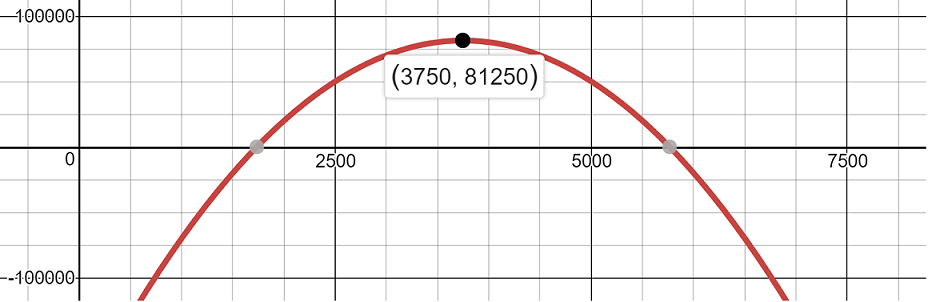
\includegraphics[scale=0.5]{extrema1new.png} \end{center}

\underline{\hspace{5in}}

Aha!  Now it's plain to see that the maximum amount of profit is achieved when $3,750$ speaker systems are produced.  According to the graph, the maximum profit that would be earned in this situation is $\$81250$.  We say that the profit function $P(x)$ has a maximum of $81250$ that is achieved at $x=3750$.  \\

Since $P(x)$ is the graph of a parabola that opens down, it should come as no surprise that the maximum profit corresponds to the vertex of the parabola.  In retrospect, answering this question didn't require a graph at all; instead, we could have used a little bit of algebra to locate the vertex.  Unfortunately, not all functions have parabolic graphs, so this technique won't always work. 

\end{explanation}
\end{example}

The above example illustrates one reason why you may want to identify the maximum of a function like $P(x)$.  You may also want to find the minimum of a function.  For example, you may want to determine how many speakers your company should produce to minimize production costs.  In this case, you would want to locate the minimum of your company's cost function.  Examples such as these motivate the next definition. 

%%Definition - Global/Absolute Maximum/Minimum.
\begin{definition}\hfil\index{maximum/minimum!global}
\begin{enumerate}
\item A function $f$ has a \dfn{global maximum} at $x=a$, if $f(a)\ge
  f(x)$ for every $x$ in the domain of the function.
\item A function $f$ has a \dfn{global minimum} at $x=a$, if $f(a)\le
  f(x)$ for every $x$ in the domain of the function.
\end{enumerate} 
A \dfn{global extremum}\index{extremum!global} is either a
global maximum or global minimum.  
\end{definition}

\begin{explanation}
Although this definition is worded formally, it is just defining the global maximum of a function, $f(x)$, to be the largest output or $f$-value that the function achieves.  If there is a maximum at $x=a$, then the function value at $x=a$, $f(a)$, will be greater than (or equal to) all of the other function values for the function, so $f(a) \geq f(x)$ for all $x$ in the domain of $f$.  \\

Similarly, if there is a global minimum of $f(x)$ at $x=a$ that means that $f(a)$ is the smallest output or $f$-value that the function achieves.  In other words, $f(a) \leq f(x)$ for all $x$ in the domain of $f$. \\
\end{explanation}

\begin{warning}
The three terms above are sometimes referred to using the word \textit{absolute} rather than global: \textit{absolute} maximum, \textit{absolute} minimum, and \textit{absolute} extremum, respectively.
\end{warning}

%%Example 1 - Abs Max, no abs min
\begin{example}
Find the global extrema of $P(x) = -0.02x^2 + 150x-200000$.
\begin{explanation}
Finding the global extrema of $P(x)$ is the same as finding the global maximum and global minimum of $P(x)$.  Let's start with the global maximum.  \\

From before, we know that the largest profit is $\$81250$, so the global maximum of $P(x)$ is $\answer{81250}$, which is achieved when $x \ = \answer{3750}$.  The domain of $P$ is $(-\infty, \infty)$ and $P(3750) = 81250 \geq P(x)$ for every $x$ in the $(-\infty, \infty)$, so our observations from before are consistent with the formal definition of global maximum. \\

\begin{explanation}

Now, let's move on to identifying the global minimum of $P$.  The global minimum occurs at $x=a$ if $P(a) \leq P(x)$ for all $x$ in the domain of $P$, which is $(-\infty, \infty)$.  Referring to the graph of $P(x)$ above, you can see that $P(x)$ \wordChoice{\choice{does}\choice[correct]{does not}} have a global minimum. 

\begin{feedback}[correct]
You got it.  We can determine that $P(x)$ has no global minimum because $P$ has no smallest output value: the $P$-values continue to decrease both as $x$ becomes very positive and as $x$ becomes very negative. 
\end{feedback}

\begin{explanation}

Let's write a quick conclusion to finish off this example. \\

On the  interval $\left( \answer{-\infty}, \answer{\infty} \right)$, the function $P(x)$ \wordChoice{\choice[correct]{is}\choice{is not}} continuous, and \wordChoice{\choice{does not have any global extrema}\choice{has a global maximum but not a global minimum}\choice{has a global minimum but not a global maximum}\choice{has both a global minimum and a global maximum}}.


\end{explanation}

\end{explanation}

\end{explanation}

\end{example}

%% Example 2 - No abs max (hole), 1 absolute min achieved twice.
\begin{exercise}
Use the graph of $y = f(x)$ below to identify the global extrema of $f$.

\begin{center} 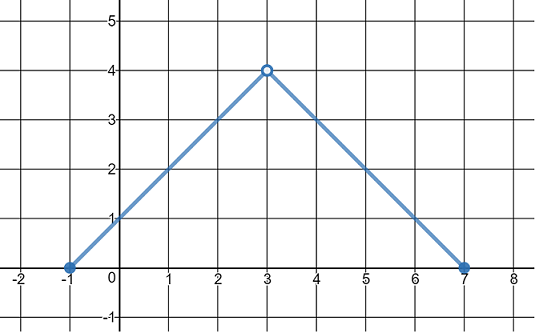
\includegraphics[scale=0.5]{extrema2new.png} \end{center}

The function $f(x)$ has an global minimum of $\answer{0}$ at $x \ = \answer{-1} \text{ and } x \ = \answer{7}$.  

\begin{exercise}
You got it!  Notice that there is only one minimum ($y=0$), and it is achieved at two distinct $x$-values $x=-1$ and $x=7$.  \\

The function $f(x)$ \wordChoice{\choice{does}\choice[correct]{does not}} have a global maximum.  

\begin{explanation}
The fact that $f$ does not have a global maximum surprises many students at first, so let's think about this a bit more.  There is a hole in the graph at the point that would correspond to a global maximum of $y=4$ if the hole were filled in.  Since there is a hole, the global maximum cannot be $y=4$ because there is no $x$ value so that $f(x) = 4$.  So what's the next highest $f$-value this function achieves?  What about $y=3.9$?  Looking at the graph, you'll notice that $f$ does achieve that $y$-value, but $f$ also achieves the bigger $y$-value $y=3.99$.  And $f$ also achieves the even bigger $y=3.999$.  You might then guess that the global maximum of $f$ is $y=3.999$, but then I could come back and point out that $f$ reaches $y=3.9999$, which is even bigger.  We could play this game forever!  The fact that we could play this game forever relies on the fact that the real numbers are \textit{dense}: given the two real numbers $3.999$ and $4$, you can always find a number $c$ such that $3.999 < c < 4$.  For example, $c = 3.9999$ would work in this case.  
\end{explanation}
\begin{exercise}
Just like we did before, let's write a quick conclusion to finish off this example. \\

On $[-1,7]$, the function $y=f(x)$ \wordChoice{\choice{is}\choice[correct]{is not}} continuous, and \wordChoice{\choice{does not have any global extrema}\choice{has a global maximum but not a global minimum}\choice{has a global minimum but not a global maximum}\choice{has both a global minimum and a global maximum}}.
\end{exercise}
\end{exercise}
\end{exercise}

%% Graph with absolute and relative extrema.
\begin{exercise}
Use the graph of $y = g(x)$ below to identify the global extrema of $g$ by filling in the blanks below. 

\begin{center} 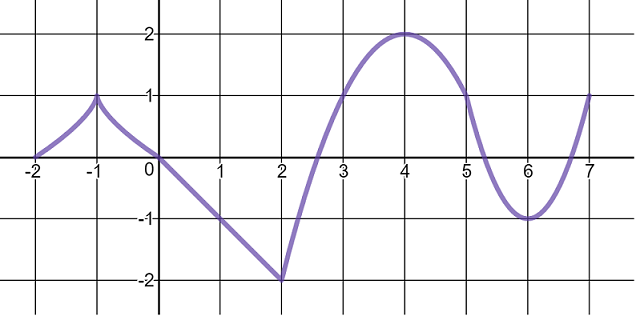
\includegraphics[scale=0.5]{extrema3new.png} \end{center}

The function $g(x)$ has a global maximum of $y \ = \answer{2}$ at $x \ = \answer{4}$ and a global minimum of $y \ = \answer{-2}$ at $x \ = \answer{2}$.

\begin{exercise}
Finally, let's write the conclusion.  \\

On the \wordChoice{\choice{open}\choice[correct]{closed}} interval $\left[ \answer{-2}, \answer{7}\right]$, the function $g(x)$ \wordChoice{\choice{does not have any global extrema}\choice{has a global maximum but not a global minimum}\choice{has a global minimum but not a global maximum}\choice{has both a global minimum and a global maximum}}.
\end{exercise}
\end{exercise}

You may have noticed in the previous example that there were $y$ values that were not the biggest $y$-values $g$ achieved on its entire domain but that were the biggest $y$-values $g$ achieved on a particular sub-interval.  For example, $y=1$ is the largest $y$-value that $g$ achieves on the interval $(-2, 1)$.  You could even say that \textit{locally} on the interval $(-2,1)$, $y=1$ is a maximum of $g$.  This is precisely what mathematicians do.  

%% Definition - Local/Relative Extrema
\begin{definition}\hfil\index{maximumminimum!local}
\begin{enumerate}
\item A function $f$ has a \dfn{local maximum} at $x=a$, if $f(a) \ge
  f(x)$ for every $x$ lying in some open interval containing $a$.
\item A function $f$ has a \dfn{local minimum} at $x=a$, if $f(a) \le
  f(x)$ for every $x$ lying in some open interval containing $a$.
\end{enumerate}
A \dfn{local extremum}\index{extremum!local} is either a local
maximum or a localinimum.
\end{definition}

\begin{explanation}
Although this definition is worded formally, it is just defining the local maximum (minimum) of a function, $f(x)$, to be the largest (smallest) output or $f$-value that the function achieves locally on some open interval.  This is precisely what we were talking about informally before the definition.
\end{explanation}

\begin{warning}
The three terms above are sometimes referred to using the word \textit{relative} rather than local: \textit{relative} maximum, \textit{relative} minimum, and \textit{relative} extremum, respectively.
\end{warning}

\begin{example}
Global maxima (minima) refer to the largest (smallest) function value that a particular function achieves globally on its entire domain.  On the other hand, local maxima (minima) refer to the largest (smallest) function value that a particular function achieves locally on some sub-interval of the real numbers, $(\infty, \infty)$.  \\

Let's think through a realistic example to help understand these terms a bit better.  If there is a woman who lives next door to you that is 6 feet, 5 inches tall, then she may very well be the tallest woman in your local neighborhood.  That means her height of 6 ft., 5 in. is a \textit{local} maximum for a person's height.  However, this woman is not the tallest person in the world!  That honor (as of 2017) goes to a Turkish man named Sultan K{\"o}sen who is 8 ft., 3 in. tall.  Across the globe, the maximum height of a person is 8 ft., 3 in., so this is the \textit{global} maximum for a person's height.  Are you starting to see the distinction between local and global?  

\end{example}

\begin{exercise}
Use the graph of $y = g(x)$ below to identify all the local extrema of $g$ by filling in the blanks below. 

\begin{center} 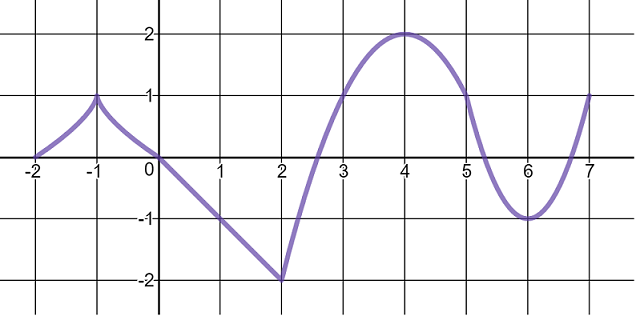
\includegraphics[scale=0.5]{extrema3new.png} \end{center}

We already know that $g$ has a global maximum of $y = 2$ at $x=4$ and an global minimum of $y=-2$ at $x=2$.  These \wordChoice{\choice[correct]{are}\choice{are not}} also local extrema.  

\begin{feedback}[correct]
You got it!  Global extrema are also local extrema.  Could you use the definitions above the justify why this is the case to a fellow classmate?  
\end{feedback}

\begin{exercise}
Whenever the domain of a function is closed (or half-closed) so that an endpoint is included in the domain of the function, you will want to investigate that endpoint when identifying relative extrema.  \\

In this case, at $x = -2$, $g$ has a local \wordChoice{\choice{maximum}\choice[correct]{minimum}} of $y \ = \answer{0}$.  \\

Also, at $x \ =\answer{7}$, $g$ has a local \wordChoice{\choice[correct]{maximum}\choice{minimum}} of $y \ = \answer{1}$.  \\

\begin{exercise}
Finally, let's identify the remaining two local extrema. \\

At $x = -1$, $g$ has a local \wordChoice{\choice[correct]{maximum}\choice{minimum}} of $y \ = \answer{1}$.  \\

At $x \ = \answer{6}$, $g$ has a local \wordChoice{\choice{maximum}\choice[correct]{minimum}} of $y \ = \answer{-1}$.  \\

\end{exercise}

\end{exercise}


\end{exercise}

\begin{warning}
Although there are a few different words used to refer to the types of extrema, on all math 160 exams we will stick to the terminology used in Thomas' calculus, 13th edition: \textit{absolute} and \textit{local} extrema.  
\end{warning}

\end{document}
